

%%%%%%%%%%%%%%%%%%%%%%%%%%%%%%%%%%%%%%%%%12pt: grandezza carattere
                                        %a4paper: formato a4
                                        %openright: apre i capitoli a destra
                                        %twoside: serve per fare un
                                        %   documento fronteretro
                                        %report: stile tesi (oppure book)
\documentclass[12pt,a4paper,openright,twoside]{report}
\usepackage{tikz}
\usepackage{amsmath, xparse}
\usetikzlibrary{matrix,chains,positioning,decorations.pathreplacing,arrows}
%
%%%%%%%%%%%%%%%%%%%%%%%%%%%%%%%%%%%%%%%%%libreria per scrivere in italiano
% \usepackage[italian]{babel}
%
%%%%%%%%%%%%%%%%%%%%%%%%%%%%%%%%%%%%%%%%%libreria per accettare i caratteri
                                        %   digitati da tastiera come è à
                                        %   si può usare anche
                                        %   \usepackage[T1]{fontenc}
                                        %   però con questa libreria
                                        %   il tempo di compilazione
                                        %   aumenta
% \usepackage[latin1]{inputenc}
%
%%%%%%%%%%%%%%%%%%%%%%%%%%%%%%%%%%%%%%%%%libreria per impostare il documento
\usepackage{fancyhdr}
%
%%%%%%%%%%%%%%%%%%%%%%%%%%%%%%%%%%%%%%%%%libreria per avere l'indentazione
%%%%%%%%%%%%%%%%%%%%%%%%%%%%%%%%%%%%%%%%%   all'inizio dei capitoli, ...
\usepackage{indentfirst}
%
%%%%%%%%%libreria per mostrare le etichette
%\usepackage{showkeys}
%
%%%%%%%%%%%%%%%%%%%%%%%%%%%%%%%%%%%%%%%%%libreria per inserire grafici
\usepackage{graphicx}
%
%%%%%%%%%%%%%%%%%%%%%%%%%%%%%%%%%%%%%%%%%libreria per utilizzare font
                                        %   particolari ad esempio
                                        %   \textsc{}
\usepackage{newlfont}
%
%%%%%%%%%%%%%%%%%%%%%%%%%%%%%%%%%%%%%%%%%librerie matematiche
\usepackage{amssymb}
\usepackage{amsmath}
\usepackage{latexsym}
\usepackage{amsthm}
%
\oddsidemargin=30pt \evensidemargin=20pt%impostano i margini
\hyphenation{sil-la-ba-zio-ne pa-ren-te-si}%serve per la sillabazione: tra parentesi 
					   %vanno inserite come nell'esempio le parole 
%					   %che latex non riesce a tagliare nel modo giusto andando a capo.

%
%%%%%%%%%%%%%%%%%%%%%%%%%%%%%%%%%%%%%%%%%comandi per l'impostazione
                                        %   della pagina, vedi il manuale
                                        %   della libreria fancyhdr
                                        %   per ulteriori delucidazioni
\pagestyle{fancy}\addtolength{\headwidth}{20pt}
\renewcommand{\chaptermark}[1]{\markboth{\thechapter.\ #1}{}}
\renewcommand{\sectionmark}[1]{\markright{\thesection \ #1}{}}
\rhead[\fancyplain{}{\bfseries\leftmark}]{\fancyplain{}{\bfseries\thepage}}
\cfoot{}
%%%%%%%%%%%%%%%%%%%%%%%%%%%%%%%%%%%%%%%%%
\linespread{1.3}                        %comando per impostare l'interlinea
%%%%%%%%%%%%%%%%%%%%%%%%%%%%%%%%%%%%%%%%%definisce nuovi comandi
%
\begin{document}
\begin{titlepage}                       %crea un ambiente libero da vincoli
                                        %   di margini e grandezza caratteri:
                                        %   si pu\`o modificare quello che si
                                        %   vuole, tanto fuori da questo
                                        %   ambiente tutto viene ristabilito
%
\thispagestyle{empty}                   %elimina il numero della pagina
\topmargin=6.5cm                        %imposta il margina superiore a 6.5cm
\raggedleft                             %incolonna la scrittura a destra
\large                                  %aumenta la grandezza del carattere
                                        %   a 14pt
%\em                                     %emfatizza (corsivo) il carattere
%Questa \`e la \textsc{Dedica}:\\
%ognuno pu\`o scrivere quello che vuole, \\
%anche nulla \ldots                      %\ldots lascia tre puntini
\newpage                                %va in una pagina nuova
%
%%%%%%%%%%%%%%%%%%%%%%%%%%%%%%%%%%%%%%%%
\clearpage{\pagestyle{empty}\cleardoublepage}%non numera l'ultima pagina sinistra
\end{titlepage}
% \pagenumbering{roman}    %serve per mettere i numeri romani
\tableofcontents
\begin{abstract}
    Il tema su cui verte questa tesi sono le attività svolte durante il tirocinio curricolare presso \emph{CNR-ISMN (Istitituto per lo Studio dei Materiali Nanostrutturati)}. \\
    L'obbiettivo del progetto svolto è stato quello di mettere in correllazione le propietà chimico/ficiche di campioni di grafene, provenienti da simulazioni al calcolatore, con
    i loro \emph{difetti} e \emph{imperfezioni} presenti nella loro struttura atomica.\\
    I sudetti \emph{difetti} infatti si presentano come dei \emph{vuoti} all'interno della struttura atomica, queste \emph{cavità} quindi sono state individuate e analizzate automaticamente utilizzando vari strumenti, fra cui la rete neurale di Object Detection \emph{YOLOv8} e la libreria di Computer Vision \emph{OpenCV}.
    Grazie a questi metodi è stato possibile andare ad analizzare automaticamente i difetti di ogni campione e cercare quindi eventuali correlazioni con le propietà fisiche del campione stesso. 
    Si è andati quindi a sviluppare una rete predittiva in grando di predire propietà chimico-fisiche a partire dalla conformazione strutturale e topologica dei campioni.
\end{abstract}

\chapter*{Introduzione}                 %crea l'introduzione (un capitolo
                                        %   non numerato)
%%%%%%%%%%%%%%%%%%%%%%%%%%%%%%%%%%%%%%%%%imposta l'intestazione di pagina
% \rhead[\fancyplain{}{\bfseries
% INTRODUZIONE}]{\fancyplain{}{\bfseries\thepage}}
% \lhead[\fancyplain{}{\bfseries\thepage}]{\fancyplain{}{\bfseries
% INTRODUZIONE}}
%%%%%%%%%%%%%%%%%%%%%%%%%%%%%%%%%%%%%%%%%aggiunge la voce Introduzione
                                        %   nell'indice
% \addcontentsline{toc}{chapter}{Introduzione}
L'Intelligenza Artificile e in particolare i modelli di Machine Learning basati sulle reti neurali nei tempi recenti si sono dimostrate tecnologie pervasive in quasi tutti gli ambiti di ricerca dimostrandosi estremamente flessibili e applicabili a domini più eternogenei e disparati. \\

Non ne fa eccezione la ricerca sui materiali innovativi come quella sul grafene, un materiale composto da un singolo strato di atomi di carbonio posizionati in conformazione esagonale dando forma ai caratteristici reticoli.
Le propietà e caratteristiche eccezionali di questo materiale derivano da molte delle sue unicità, quali per esempio il suo sottilissimo spessore lungo solo un atomo e quindi il suo peso estremamente contenuto. \\
Queste propietà \emph{bidimensionali} conferiscono al materiale resistenza, flessibilità e leggerezza senza concorrenza tra gli altri materiali tradizionali. \\
Le possibili applicazioni di un simile materiale sono anchesse estramamente multi-dominio e spaziano dai supercondensatori, semiconduttori, nonchè per usi strutturali e tanto altro. 
Per la natura stessa del materiale, la produzione su scala industriale risulta tutt'altro che banale e i costi elevati. \\
Spesso durante la produzione non si riesce ad ottenere un campione di grafene perfetto totalmente privo di impurità. E' inoltre possibile trovare danni strutturali sul reticolo di carbonio con conseguente presenza di cavità sullo stesso. \\

L'idea del progetto quindi si è basata sull'analisi di campioni di grafene difettato derivante da simulazioni. Grazie alla conoscenza a priori delle propietà fisiche di ogni campione, originariamente calcolate dalle simulazioni è stato possibile mettere in correlazione la topologia e i tratti geomtrici dei suddetti difetti con le propietà del materiale stesso.\\
In primo luogo, prima di andare ad analizzare le geometrie dei vari difetti è risultato utile individuarli automaticamente. 
Questo è stato fatto addestrando la rete neurale YOLOv8, potente modello di Object Detection noto per la sua velocità di inferenza e per le elevate performace otenibili dopo un training relativaemnte breve e con campioni limitati.\\
Una volta individuate ed estratte dallo sfondo le regioni di interesse si è proceduto con l'analisi geomtrica e topologica dei difetti con la libreria di Computer Vision OpenCV.
Questa libreria multipiattaforma inizialmente sviluppata da Intel e divenuta successivamente open-source offre numerose funzioni e metodi per applicazioni di computer vision, nel caso di questo progetto ci si è intereafacciati ad essa tramite Python. \\
E' stato quindi possibile grazie ad essa estrapolare tratti geometrici e topologici dai difetti in questione calcolando tratti più semplici come area, perimetro fino a quelli più sofisticati quali eccenticità, circolarità e molto altro.\\
I dati sono stati integrati in un dataframe Pandas, grazie ad esso sono state fatte analisi sulle correlazioni fra i parametri stessi. Trovare parametri molto correlati fra loro è importante per evitare di selezionare valori ridondanti nell'addestramento della rete predittiva.\\

(Addestramento rete predittiva -- work in progress)
%%%%%%%%%%%%%%%%%%%%%%%%%%%%%%%%%%%%%%%%%non numera l'ultima pagina sinistra
\clearpage{\pagestyle{empty}\cleardoublepage}
%%%%%%%%%%%%%%%%%%%%%%%%%%%%%%%%%%%%%%%%%imposta l'intestazione di pagina
\rhead[\fancyplain{}{\bfseries\leftmark}]{\fancyplain{}{\bfseries\thepage}}
\lhead[\fancyplain{}{\bfseries\thepage}]{\fancyplain{}{\bfseries
INDICE}}
% %%%%%%%%%%%%%%%%%%%%%%%%%%%%%%%%%%%%%%%%%non numera l'ultima pagina sinistra
% \clearpage{\pagestyle{empty}\cleardoublepage}
% \listoffigures                          %crea l'elenco delle figure
% %%%%%%%%%%%%%%%%%%%%%%%%%%%%%%%%%%%%%%%%%non numera l'ultima pagina sinistra
% \clearpage{\pagestyle{empty}\cleardoublepage}
% \listoftables                           %crea l'elenco delle tabelle
% %%%%%%%%%%%%%%%%%%%%%%%%%%%%%%%%%%%%%%%%%non numera l'ultima pagina sinistra
% \clearpage{\pagestyle{empty}\cleardoublepage}
\chapter{Introduzione al Machine Learning}                %crea il capitolo
%%%%%%%%%%%%%%%%%%%%%%%%%%%%%%%%%%%%%%%%%imposta l'intestazione di pagina
\lhead[\fancyplain{}{\bfseries\thepage}]{\fancyplain{}{\bfseries\rightmark}}
\pagenumbering{arabic}                  %mette i numeri arabi
La disciplina di ricerca sull'Intelligenza artificale pone le sue radici già a metà del XX secolo. L'obbiettivo generale di allora era quello di sviluppare macchine capaci di eseguire mansioni tipicamente attribute e svolte da umani. 
Con il passare dei decenni l'obbiettivo è rimasto lo stesso ma si sono esplorate numerose vie e teniche differenti anche molto diverse tra loro, fra cui la sottocatgoria denominata come \emph{Machine Learning}. Quest'ultima è l'insieme delle tecniche e dei metodi statistici con i quali si va migliorare un algoritmo che ha come obbiettivo quello di identificare pattern nei dati. 
Questi metodi si sono riveati particolarmente utili in quei campi dove è notoriamente difficile se non impossibile sviluppare soluzioni tramite algoritmi tradizionali, per esempio il riconoscimento vocale e di immagini.\\
Negli ultimi decenni con il rapido avanzamento della velocità di calcolo a disposizione queste tecnologie hanno ricevuto una notevole accellerazione nello sviluppo e nei risultati raggiunti. 
In particolare ha preso sempre più popolarità l'approcio denomicanto come Deep Learning ovvero quei metodi basati su reti neurali artificiali su più livelli. Ognuno di questi livelli estrapola gerarchie di inforamzioni di più alto livello definite a loro volta su quelle di livello inferiore calcolate dagli strati precedenti.
\section{Reti neurali}
\subsection{Architettura }%crea la sezione
Una rete neurale consiste in un insieme di \emph{neuroni} (detti anche \emph{nodi}) collegati fra loro, che concorrono per risolvere un problema.
Ogni nodo può essere pensato come una semplice funzione di tante variabili di ingresso quanti sono i nodi collegati ad esso. \\
Il suo valore di attivazione quindi sarà la somma pesata dei valori di attivazione dei nodi che prende come input, più la somma di un valore chiamato \emph{bias}, il tutto all’interno di una \emph{funzione di attivazione} non lineare. \\
In formule l’attivazione di un neurone può essere espressa dalla semplice formula: \\
\begin{equation}
    y = \sigma(w \cdot x + b)
\end{equation}
Dove, \\
\begin{itemize}
    \item 
        $y$ è il valore scalare di attivazione del nodo, esso può variare con continuità da 0 a 1, dove 0 rappresenta la totale assenza di attivazione del nodo, mentre 1 rappresenta l'attivazione massima possibile. 
    \item 
        $ x= \begin{bmatrix} x_1 , x_2 , \cdot\cdot , x_n\end{bmatrix} $ rappresenta il vettore di input, ovvero i valori di attivazione $x_1, x_2, ... , x_n$ degli $n$ neuroni connessi al neurone in questione.
    \item 
        $ w= \begin{bmatrix} w_1 , w_2 , \cdot\cdot , w_n\end{bmatrix} $ della stessa dimensione di $x$
        reppresenta il vettore dei $pesi$, questi parametri sono importanti in quanto venendo moltiplicati per i rispettivi valori di input permettono di calcolare la media pesata dei valori di ingresso.
    \item 
        $b$ è detto $bias$, un valore che si va a sommare semplicemente alla somma pesata degli input.
    \item 
        $\sigma$ è la \emph{funzione di attivazione}, ne esistono di numerosi tipi, il suo compito principale è quello di aggiungere una componente di \emph{non-linearità} alla rete stessa. 

\end{itemize}
 Graficamente l'attivazione di un nuerone con soli tre input può essere rappresentata come: \\
 \begin{center}
     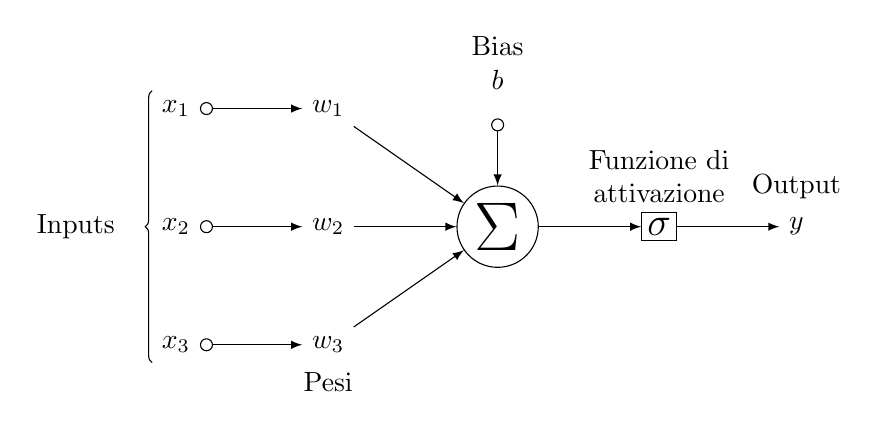
\begin{tikzpicture}[
init/.style={
  draw,
  circle,
  inner sep=2pt,
  font=\Huge,
  join = by -latex
},
squa/.style={
  draw,
  inner sep=2pt,
  font=\Large,
  join = by -latex
},
start chain=2,node distance=13mm
]
\node[on chain=2] 
  (x2) {$x_2$};
\node[on chain=2,join=by o-latex] 
  {$w_2$};
\node[on chain=2,init] (sigma) 
  {$\displaystyle\Sigma$};
\node[on chain=2,squa,label=above:{\parbox{2cm}{\centering Funzione di \\ attivazione}}]   
  {$\sigma$};
\node[on chain=2,label=above:Output,join=by -latex] 
  {$y$};
\begin{scope}[start chain=1]
\node[on chain=1] at (0,1.5cm) 
  (x1) {$x_1$};
\node[on chain=1,join=by o-latex] 
  (w1) {$w_1$};
\end{scope}
\begin{scope}[start chain=3]
\node[on chain=3] at (0,-1.5cm) 
  (x3) {$x_3$};
\node[on chain=3,label=below:Pesi,join=by o-latex] 
  (w3) {$w_3$};
\end{scope}
\node[label=above:\parbox{2cm}{\centering Bias \\ $b$}] at (sigma|-w1) (b) {};

\draw[-latex] (w1) -- (sigma);
\draw[-latex] (w3) -- (sigma);
\draw[o-latex] (b) -- (sigma);

\draw[decorate,decoration={brace,mirror}] (x1.north west) -- node[left=10pt] {Inputs} (x3.south west);
\end{tikzpicture}
 \end{center}

Sempre in formule si può rappresentare l'attivazione del neurone in forma estesa come: 
\begin{equation}
    y = \sigma(w_1  x_1 + w_1  x_1 + .. w_n  x_n + b) = \sigma(\sum_{n=1}^{n} w_n x_n + b)
\end{equation}
La funzione di attivazione è necessaria innanzitutto per trasformare un valore \emph{unbunded}, ovvero senza un valore massimo, derivante dalla sommatoria degli input in un valore continuo che va da 0 a 1, ovvero il valore di attivazione finale che vogliamo fare assumere al neurone del caso. \\
Esistono numerose funzioni di attivazione, una delle più famose e semplici è la \emph{Sigmoide} \[ S(x) = \frac{1}{1+e^{-x}}\] simile alla funzione \emph{gradino unitario} ma in versione smussata, senza la discontinuità nello zero. Questa funzione rispetto al \emph{gradino unitario} ha vari vantaggi, in particolare a piccole variazioni dell'input avremo piccole variazioni nell'output. \\
Nelle reti più moderne è sempre più utilizzata la RELU, ovvero la funzione rettificatore espressa semplicemente come: 
\begin{equation}
     f(x)=\max(0,x)
\end{equation}
Quest'ultima si è dimostrata come la più efficace nelle reti di apprendimento profondo. Fra i suoi vantaggi abbiamo l'attivaazione scarsa, infatti essa si attiva solo nella metà dei campioni di una rete inizializzata casualmente inoltre si hanno meno problemi in fase di discesa del gradiente nella fase di adestramento rispetto alla funzione Sigmoide dei quali parleremo più avanti nel capitolo.
\begin{figure}[h]
\begin{minipage}[t]{0.49\linewidth}
\centering
\includegraphics[width=\linewidth]{gradino.png}

(a) Gradino unitario
\end{minipage}%
\hfill\vrule\hfill
\begin{minipage}[t]{0.49\linewidth}
\centering
\includegraphics[width=\linewidth]{sigmoid.png}

(b)  Sigmoide
\end{minipage}
\caption{Comparazione fra funzione gradino unitario e sigmoide }
\end{figure}

Esistono poi funzioni di attivazione più sofisticate, come la Softmax.
Quest'ultima è spesso utile nelle reti classificatrici multiclasse. In questi casi i nodi del layer di output rappesentano la probabilità di classificazione per ciascuna classe la sommatoria dei valori di attivazione dei nodi dell'ultimo layer deve fare necessariamente 1.
\newpage
Nel caso generale abbiamo almeno un layer di nodi di input uno di output e acluni layer intermedi detti \emph{hidden-layer},
in una rete \emph{fully-connected} tutti i nodi nell n-esimo layer sono connessi a tutti i nodi dell'n-esimo layer. \\
Le feature dei vari pattern estrapolati dalla rete vengono propio calcolati dai layer interni i quali estrapolano propietà sempre più astratte e di alto livello quanto è avanzata la posizione del layer in cui risiedono. \\
Il vettore dei valori di attivazione del primo \emph{hidden-layer} può essere espresso come il prodotto tra la matrice dei pesi del layer corrente e il vettore di attivazione del layer precedente più il vettore dei bias, tutto dentro la funzione di attivazione scelta per quel layer.

\begin{figure}[h]
\centering
\includegraphics[width=\linewidth]{neural_networks-004.png}
\caption{Rete neurale \emph{fully-connected} con $3$ \emph{hidden layers} da $m$ nodi ciascuno.}
\end{figure}

\newpage
In formule il vettore dei valori di attivazione del primo \emph{hidden-layer} può essere espresso come:
    \begin{equation} 
     \begin{pmatrix}
        a_{1}^{(1)} \\[0.3em]
        a_{2}^{(1)} \\
        \vdots \\
        a_{m}^{(1)}
      \end{pmatrix}
    =
      \sigma \left[ 
      \begin{pmatrix}
        w_{1,0} & w_{1,1} & \ldots & w_{1,n} \\
        w_{2,0} & w_{2,1} & \ldots & w_{2,n} \\
        \vdots  & \vdots  & \ddots & \vdots  \\
        w_{m,0} & w_{m,1} & \ldots & w_{m,n}
      \end{pmatrix}
      {
      \begin{pmatrix}
        a_{1}^{(0)} \\[0.3em]
        a_{2}^{(0)} \\
        \vdots \\
        a_{n}^{(0)}
      \end{pmatrix}}
      +
      \begin{pmatrix}
        b_{1}^{(0)} \\[0.3em]
        b_{2}^{(0)} \\
        \vdots \\
        b_{m}^{(0)}
      \end{pmatrix}\right] 

      \\
    \end{equation}
In notazione compatta abbiamo: 
    \begin{equation}
        \mathbf{a}^{(1)} = \mathbf{W}^{(0)} {a^{(0)}}+\mathbf{b}^{(0)}
    \end{equation}

In generale non tutti le reti sono \emph{fully-connected}, spesso si opta per una soluzione ibrida dove si utilizzano strati con architetture diverse per risolvere un problema. 
Un esempio di un'altra archiettura di rete sono le reti ricorsive (RNN), queste hanno dei collegamenti in retroazione capaci di mantenere uno \emph{stato} e quindi avere \emph{memoria}. Mantenere una memoria è cruciale quando gli imput passati in precedenza nella rete in relazione con quelli attuali hanno un significato semantico importante, come per esempio nell'analisi di un video o per un riconoscimento vocale partendo da un file audio.
Un'altro tipo di rete molto importante e centrale in questo lavoro di tesi sono le reti convoluzionali CNN. Esse si basano su filtri convoluzionali che collegano gli \emph{hidden-layer}.\\
Questo tipo di reti sono state usate nell'ambito di questo progetto per identificare aumaticamente le aree di interesse dove sono presenti i difetti del grafene. Di queste reti e in particolare YOLOv8 ne parleremo nel dettaglio nel prossimo capitolo.

\newpage
\section{Funzione di costo e algoritmi di apprendimento}
Uno dei parametri più importanti nonchè alla base degli algoritmi di apprendimento è la cosidetta \emph{funzione di costo}.
Ne esistono di vari tipi ma intuitivamente essa è una funzione reale che prende come variabili i parametri del sistema $C(\mathbf{W,b})$, quindi da un'indicazione su quanto bene la nostra rete stia performando sui campioni che gli vengono forniti.\\
Questa valutazione è possibile confrontando i valori $y(x)$ che la rete produce per gli imput $x$ conoscendo il vettore $a(x)$ dei risultati attesi per gli imput in questione.
Una delle più utilizzate è lo \emph{scarto quadratico medio}, essa fa la media aritmetica del quadrato dell'errore di output rispetto a ogni imput.
\begin{equation}
    C(\mathbf{W,b}) = \frac{1}{n} \sum_{n=1}^{n} (y(x_{i}) - a_{i}))^2
\end{equation}

Al variare dei numerosi parametri $(W,b)$ la performance della rete varia e così anche la funzione di costo. In particolare più il valore si avvicina a zero e più la rete sta performando bene. \\
Risulata quindi chiaro che minimizzare la funzione di costo $C(\mathbf{W,b})$ è il fulcro del problema dell'addestramento delle reti neurali.
\subsection{Discesa del gradiente}
Siamo quindi di fronte a un problema di ottimizzazione di una funzione reale in tante variabili quanti sono i parametri della rete, dove si cerca quindi un minimo della funzione stessa.
Intuitivamente l'inverso del gradiente ci da un'indicazione \emph{spaziale} su dove dobbiamo muoverci per avvicinarci il più velocemente possibile a più vicino minimo locale, quindi per quale vettore di valori dobbiamo sommare i nsotri parametri per migliorarli. \\
% Com'è logico aspettarsi non è possibile visualizzare graficamente questa discesa a causa delle dimensioni del nostro spazio (pari al numero dei parametri).
% Semplificando al massimo e considerando solo due parametri è possibile comunque osservare il procedimento di discesa del gradiente nella seguente immagine: 

% \begin{figure}[h]
% \centering
% \includegraphics[width=\linewidth]{800px-Gradient_descent.svg.png}
% \caption{Esempio di discesa del gradiente verso un minimo nel caso di soli due parametri.}
% \end{figure}
% \newpage

Le iterazioni del metodo si presentano nella forma seguente, dove vado a calcolare l'inverso del gradiente per poi sommarlo ai vecchi parametri, in questo modo vado ad ottenere i nuovi parametri. \\
L'equzione seguente mostra un'iterazione del processo di discesa del gradiente, dove vengono calcolati i nuovi parametri $(\omega', b')$:
\begin{equation}
    (\omega', b') := (w,b)-\eta \nabla C(w,b)
\end{equation}
Importante notare come l'entità dello \emph{spostamento} per ogni step è arbitrariamente piccola rispetto al valore di $\eta$. Quest'ultimo prende il nome di \emph{learning-rate} ed è un \emph{iperparametro} in quanto è una variabile scelta a priori da colui che sta addestrando la rete. \\
Un'altro accorgimento per evitare fluttuazioni imprevedibili dei parametri è quello di non applicare i cambiamenti ad ogni predizione ma fare la media su un batch di più predizioni. \\
Il metodo illustrato sopra prende il nome di \emph{Gradient Descent GD}, questo è un metodo applicabile quando la funzione di costo è sufficientemente semplice e il suo gradiente è di facile computazione.\\
Nel GD si calcola il gradiente per l'intero set di parametri ed essi vengono aggiornati ad ogni iterazione. \\
Quando invece ho dataset molto grandi oppure non ho un'espressione della funzione di costo abbastanza semplice si può optare per il metodo noto come \emph{Stochastic Gradient Descent SGD}.
Questo metodo approssima il calcolo del gradiente considerando ogni volta un batch casuale di paramertri ad ogni iterazione.

\begin{figure}[h]
\centering
\includegraphics[width=\linewidth]{Stogra.png}
\caption{Esempio di andamento della funzione costo nel corso delle iterazioni in un problema di ottimizzazione risolto tramite SGD}
\end{figure}
\newpage
Come si può vedere dall'andamento della funzione di costo durante le iterazioni del SGD, non è assicurato il miglioramento della rete ad ogni iterazione, in alcuni casi infatti la funzione di costo può momentaneamente salire, questo è dovuto alla natura stocastica, quindi probabilistica del metodo.\\
In generale comunque per computare la derivata parizale di un parametro occorre un passaggio e il tutto deve essere ripetuto per ogni epoca. \\
Avendo spesso miliardi di parametri e centinaia di epoche i metodi di GD possono risultare facilemente costosi computazionalemente. \\
Per mitigare questo è stato creato un nuovo algoritmo utilizzabile insieme al SGD, esso prende il nome di \emph{Backpropagation}.
Questo algoritmo ricorsivo sfruttando la regola della \emph{chain rule} (durante il calcolo delle derivate parziali del gradiente) permette di calcolare tutte le derivate e quindi l'intero gradiente in un singolo passaggio.\\

Qui sotto mostro la differenza intuitiva fra la progressione di un algoritmo di GD a batch con uno di SGD.\\
Notare bene come la visualizzazione è possibile solo se si considera il caso estremamente semplificato di soli due parametri. \\Nel caso generico con più di due parametri (anche miliardi) sarebbe impossibile proporre una visualizzazione di uno spazio con così tante dimensioni.

\begin{figure}[h]
\begin{minipage}[t]{0.49\linewidth}
\centering
\includegraphics[width=\linewidth]{batchGD.png}

(a) Batch Gradient Descent
\end{minipage}%
\hfill\vrule\hfill
\begin{minipage}[t]{0.49\linewidth}
\centering
\includegraphics[width=\linewidth]{SGD.png}

(b)  Stochastic Gradient Descent
\end{minipage}
\caption{Comparazione fra iterazioni di GD a batch e SGD }
\end{figure}

Notare la natura intrisecamente probabilistica degli step del SGD, essi non assicurano un miglioramento della loss ad ogni step ma il risulato finale può risultare comunque più efficente della controparte GD se analizzato nel complesso.



% \subsection{Algoritmi di apprendimento}
% \clearpage{\pagestyle{empty}\cleardoublepage}
% %%%%%%%%%%%%%%%%%%%%%%%%%%%%%%%%%%%%%%%%%per fare le conclusioni
% \chapter*{Conclusioni}
% %%%%%%%%%%%%%%%%%%%%%%%%%%%%%%%%%%%%%%%%%imposta l'intestazione di pagina
% \rhead[\fancyplain{}{\bfseries
% CONCLUSIONI}]{\fancyplain{}{\bfseries\thepage}}
% \lhead[\fancyplain{}{\bfseries\thepage}]{\fancyplain{}{\bfseries
% CONCLUSIONI}}
% %%%%%%%%%%%%%%%%%%%%%%%%%%%%%%%%%%%%%%%%%aggiunge la voce Conclusioni
%                                         %   nell'indice
% \addcontentsline{toc}{chapter}{Conclusioni} Queste sono le
% conclusioni.\\
% In queste conclusioni voglio fare un riferimento alla
% bibliografia: questo \`e il mio riferimento \cite{K3,K4}.
% %%%%%%%%%%%%%%%%%%%%%%%%%%%%%%%%%%%%%%%%%imposta l'intestazione di pagina
% \renewcommand{\chaptermark}[1]{\markright{\thechapter \ #1}{}}
% \lhead[\fancyplain{}{\bfseries\thepage}]{\fancyplain{}{\bfseries\rightmark}}
% \appendix                               %imposta le appendici
% \chapter{Prima Appendice}               %crea l'appendice
% In questa Appendice non si \`e utilizzato il comando:\\
% %%%%%%%%%%%%%%%%%%%%%%%%%%%%%%%%%%%%%%%%%\verb"" è equivalente all'
%                                         %   ambiente verbatim,
%                                         %   ma si utilizza all'interno
%                                         %   di un discorso.
% \verb"\clearpage{\pagestyle{empty}\cleardoublepage}", ed infatti
% l'ultima pagina 8 ha l'intestazione con il numero di pagina in
% alto.
% %%%%%%%%%%%%%%%%%%%%%%%%%%%%%%%%%%%%%%%%%imposta l'intestazione di pagina
% \rhead[\fancyplain{}{\bfseries \thechapter \:Prima Appendice}]
% {\fancyplain{}{\bfseries\thepage}}
% \chapter{Seconda Appendice}             %crea l'appendice
% %%%%%%%%%%%%%%%%%%%%%%%%%%%%%%%%%%%%%%%%%imposta l'intestazione di pagina
% \rhead[\fancyplain{}{\bfseries \thechapter \:Seconda Appendice}]
% {\fancyplain{}{\bfseries\thepage}}
% \begin{thebibliography}{90}             %crea l'ambiente bibliografia
% \rhead[\fancyplain{}{\bfseries \leftmark}]{\fancyplain{}{\bfseries
% \thepage}}
% %%%%%%%%%%%%%%%%%%%%%%%%%%%%%%%%%%%%%%%%%aggiunge la voce Bibliografia
%                                         %   nell'indice
% \addcontentsline{toc}{chapter}{Bibliografia}
% %%%%%%%%%%%%%%%%%%%%%%%%%%%%%%%%%%%%%%%%%provare anche questo comando:
% %%%%%%%%%%%\addcontentsline{toc}{chapter}{\numberline{}{Bibliografia}}
% \bibitem{K1} Primo oggetto bibliografia.
% \bibitem{K2} Secondo oggetto bibliografia.
% \bibitem{K3} Terzo oggetto bibliografia.
% \bibitem{K4} Quarto oggetto bibliografia.
% \end{thebibliography}
% %%%%%%%%%%%%%%%%%%%%%%%%%%%%%%%%%%%%%%%%%non numera l'ultima pagina sinistra
% \clearpage{\pagestyle{empty}\cleardoublepage}
% \chapter*{Ringraziamenti}
% \thispagestyle{empty}
% Qui possiamo ringraziare il mondo intero!!!!!!!!!!\\
% Ovviamente solo se uno vuole, non \`e obbligatorio.
\end{document}
